\documentclass{standalone}
\usepackage{tikz}
\usepackage{ctex,siunitx}
\setCJKmainfont{Noto Serif CJK SC}
\usepackage{tkz-euclide}
\usepackage{amsmath}
\usetikzlibrary{patterns, calc}
\usetikzlibrary {decorations.pathmorphing, decorations.pathreplacing, decorations.shapes,}

\begin{document}
\small
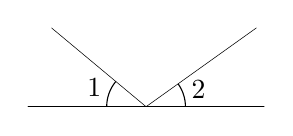
\begin{tikzpicture}[>=stealth,scale=1]
  \tkzSetUpPoint[fill=black]
  % \useasboundingbox(-1,-0.75)rectangle(3.7,1.4);
  \tkzDefPoints{-1.5/.5/A, 1.5/.5/B, 0/.5/O, -1.2/1.5/A', 1.4/1.5/B'}
  \tkzDrawSegments(A,B O,A' O,B')
  \tkzMarkAngles[mark=none, size=.5](A',O,A B,O,B')
  \tkzLabelAngle[pos=.7](A',O,A){1}
  \tkzLabelAngle[pos=.7](B,O,B'){2}
\end{tikzpicture}
\end{document}